
%%%%%%%%%%%%%%%%%%%%%%%%%%%%%%%%%%%%%%%%%%%%%%%%%%%%%%%%
%
% Copyright (c) 2003-2010 by University of Queensland
% Earth Systems Science Computational Center (ESSCC)
% http://www.uq.edu.au/esscc
%
% Primary Business: Queensland, Australia
% Licensed under the Open Software License version 3.0
% http://www.opensource.org/licenses/osl-3.0.php
%
%%%%%%%%%%%%%%%%%%%%%%%%%%%%%%%%%%%%%%%%%%%%%%%%%%%%%%%%

\section{Steady-state Heat Refraction}
\label{STEADY-STATE HEAT REFRACTION}

In this chapter we demonstrate how to handle more complex geometries. 

Steady-state heat refraction will give us an opportunity to investigate some of
the richer features that the \esc package has to offer. One of these is \pycad .
The advantage of using \pycad is that it offers an easy method for developing
and manipulating complex domains. In conjunction with \gmsh we can generate
finite element meshes that conform to our domain's shape providing accurate
modelling of interfaces and boundaries. Another useful function of \pycad is
that we can tag specific areas of our domain with labels as we construct them.
These labels can then be used in \esc to define properties like material
constants and source locations. 

We proceed in this chapter by first looking at a very simple geometry. Whilst a
simple rectangular domain is not very interesting the example is elaborated upon
later by introducing an internal curved interface.

\begin{figure}[ht]
\centerline{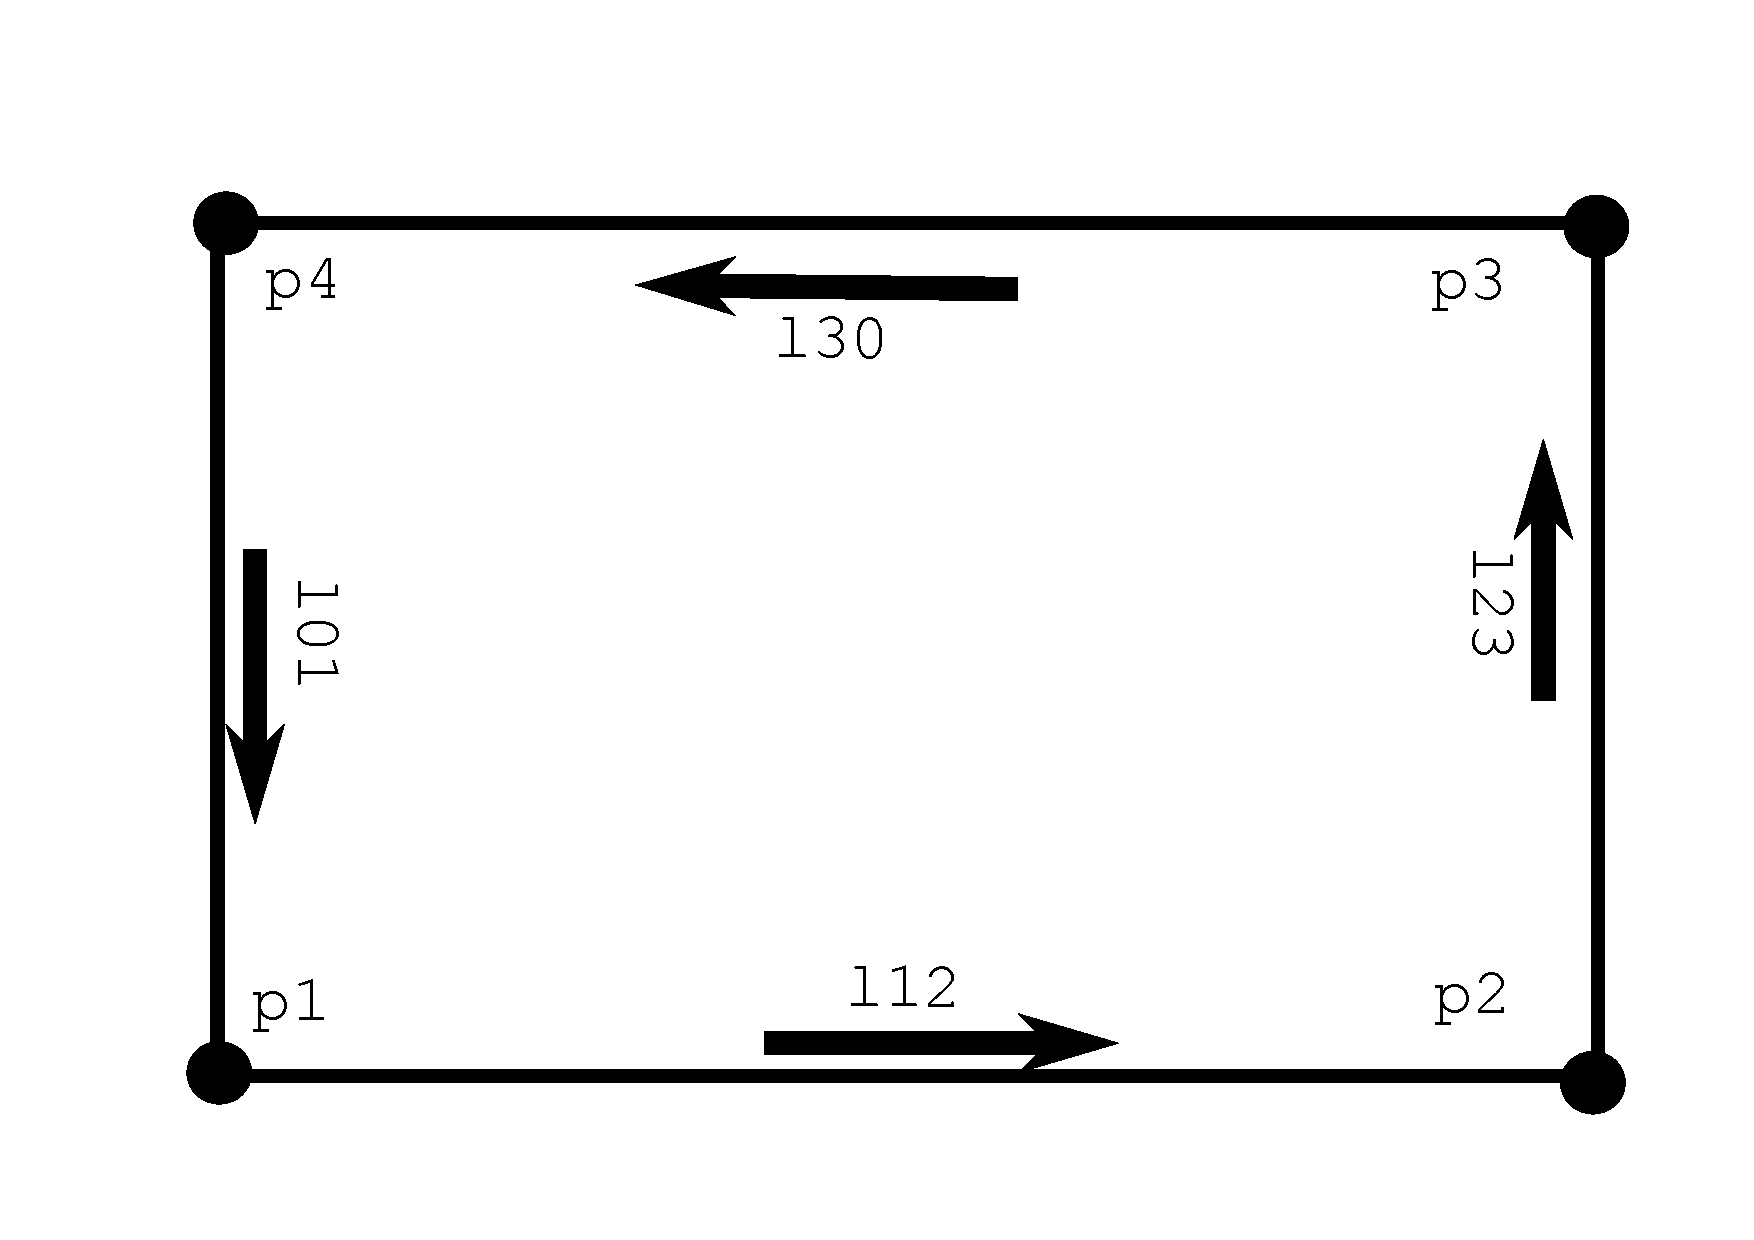
\includegraphics[width=4.in]{figures/pycadrec}}
\caption{Example 4: Rectangular Domain for \pycad.}
\label{fig:pycad rec}
\end{figure}

\section{Example 4: Creating the domain with \pycad}
\label{example4}
\sslist{example04a.py}

We modify the example in Chapter~\ref{CHAP HEAT 2a} in two ways: we look the
steady state 
case with slightly modified boundary conditions and use a more flexible tool 
to generate to generate the geometry. Lets look at the geometry first. 

We want to define a rectangular domain of width $5 km$ and depth $6 km$ below
the surface of the Earth. The domain is subject to a few conditions. The
temperature is known at the surface and the basement has a known heat flux. Each
side of the domain is insulated and the aim is to calculate the final
temperature distribution.

In \pycad there are a few primary constructors that build upon each other to
define domains and boundaries; 
the ones we use are:
\begin{python}
from esys.pycad import *
Point() #Create a point in space.
Line() #Creates a line from a number of points.
CurveLoop() #Creates a closed loop from a number of lines.
PlaneSurface() #Creates a surface based on a CurveLoop
\end{python}
So to construct our domain as shown in \reffig{fig:pycad rec}, we first need to
create
the corner points. From the corner points we build the four edges of the
rectangle. The four edges
then form a closed loop which defines our domain as a surface.
We start by inputting the variables we need to construct the model.
\begin{python}
width=5000.0*m   #width of model
depth=-6000.0*m  #depth of model
\end{python} 
The variables are then used to construct the four corners of our domain, which
from the origin has the dimensions of 5000 meters width and -6000 meters depth.
This is done with the \verb Point()  function which accepts x, y and z
coordinates. Our domain is in two dimensions so z should always be zero. 
\begin{python}
# Overall Domain
p0=Point(0.0,      0.0, 0.0)
p1=Point(0.0,    depth, 0.0)
p2=Point(width, depth, 0.0)
p3=Point(width,   0.0, 0.0)
\end{python}
Now lines are defined using our points. This forms a rectangle around our
domain;
\begin{python}
l01=Line(p0, p1)
l12=Line(p1, p2)
l23=Line(p2, p3)
l30=Line(p3, p0)
\end{python}
Notice that lines have a direction. These lines form the basis for our domain
boundary, which is a closed loop.
\begin{python}
c=CurveLoop(l01, l12, l23, l30)
\end{python}
Be careful to define the curved loop in an \textbf{anti-clockwise} manner
otherwise the meshing algorithm may fail.
Finally we can define the domain as
\begin{python}
rec = PlaneSurface(c)
\end{python}
At this point the introduction of the curved loop seems to be unnecessary but
this concept plays an important role 
if holes are introduced. 

Now we are ready to handover the domain \verb|rec| to a mesher which subdivides
the domain into triangles (or tetrahedron in 3D). In our case we use \gmsh. We
create 
an instance of the \verb|Design| class which will handle the interface to
\gmsh: 
\begin{python}
from esys.pycad.gmsh import Design 
d=Design(dim=2, element_size=200*m)
\end{python}
The argument \verb|dim| defines the spatial dimension of the domain\footnote{If
\texttt{dim}=3 the rectangle would be interpreted as a surface in the three
dimensional space.}. The second argument \verb|element_size| defines element
size which is the maximum length of a triangle edge in the mesh. The element
size needs to be chosen with care in order to avoid very dense meshes. If the
mesh is too dense, the computational time will be long but if the mesh is too
sparse, the modelled result will be poor. In our case with an element size of
$200$m 
and a domain length of $6000$m we will end up with about $\frac{6000m}{200m}=30$
triangles in each spatial direction. So we end up with about $30 \times 30 =
900$ triangles which is a size that can be handled easily.
We can easily add our domain \verb|rec| to the \verb|Design|;
\begin{python}
d.addItem(rec)
\end{python}
We have the plan to set a heat flux on the bottom of the domain. One can use the
masking technique to do this
but \pycad offers a more convenient technique called tagging. With this
technique items in the domain are
named using the \verb|PropertySet| class. We can then later use this name to set
values secifically for
those sample points located on the named items. Here we name the bottom face of
the 
domain where we will set the heat influx:
\begin{python}
ps=PropertySet("linebottom",l12))
d.addItem(ps)
\end{python}
Now we are ready to hand over the \verb|Design| to \FINLEY:
\begin{python}
from esys.finley import MakeDomain
domain=MakeDomain(d)
\end{python}
The \verb|domain| object can now be used in the same way like the return object
of the \verb|Rectangle| 
object we have used previously to generate a mesh. It is common practice to
separate the 
mesh generation from the PDE solution. The main reason for this is that mesh
generation can be computationally very expensive in particular in 3D. So it is
more efficient to generate the mesh once and write it to a file. The mesh
can then be read in every time a new simulation is run. \FINLEY supports this in
the following 
way~\footnote{An alternative are the \texttt{dump} and \texttt{load} functions.
They using a binary format and tend to be much smaller.}
\begin{python}
# write domain to an text file
domain.write("example04.fly")
\end{python}
and then for reading in another script;
\begin{python}
# read domain from text file
from esys.finley import ReadMesh
domain =ReadMesh("example04.fly")
\end{python}

\begin{figure}[ht]
\centerline{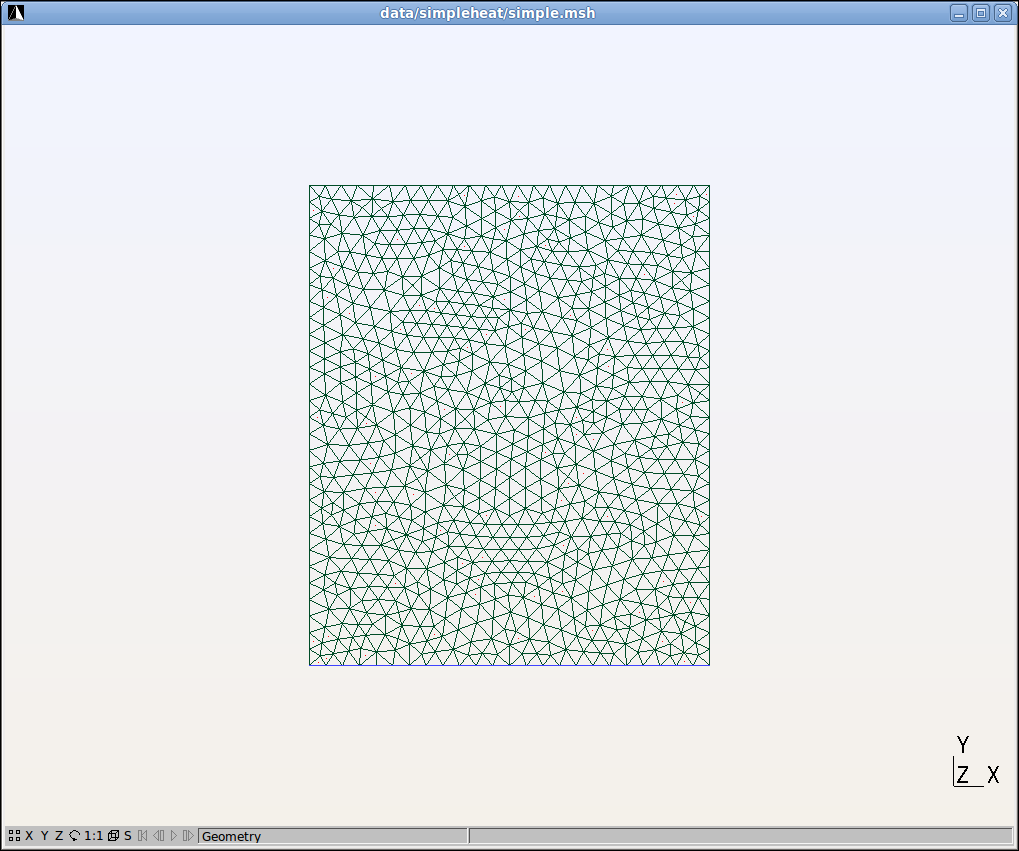
\includegraphics[width=4.in]{figures/simplemesh}}
\caption{Example 4a: Mesh over rectangular domain, see \reffig{fig:pycad rec}.}
\label{fig:pycad rec mesh}
\end{figure}

Before we discuss how to solve the PDE for this 
problem, it is useful to present two additional options of the \verb|Design|
class. 
They allow the user accessing the script which is used by \gmsh to generate the
mesh as well as
the mesh as it has been generated by \gmsh. This is done by setting specific
names for these files: 
\begin{python}
d.setScriptFileName("example04.geo")
d.setMeshFileName("example04.msh")
\end{python}
Usually the extension \texttt{geo} is used for the script file of the \gmsh
geometry and
the extension \texttt{msh} for the mesh file. Normally these files are deleted
after usage. 
Accessing these files can be helpful to debug the generation of more complex
geometries. The geometry and the mesh can be visualised from the command line
using
\begin{verbatim}
gmsh example04.geo  # show geometry
gmsh example04.msh  # show mesh
\end{verbatim}
The mesh is shown in \reffig{fig:pycad rec mesh}.
\begin{figure}[ht]
\centerline{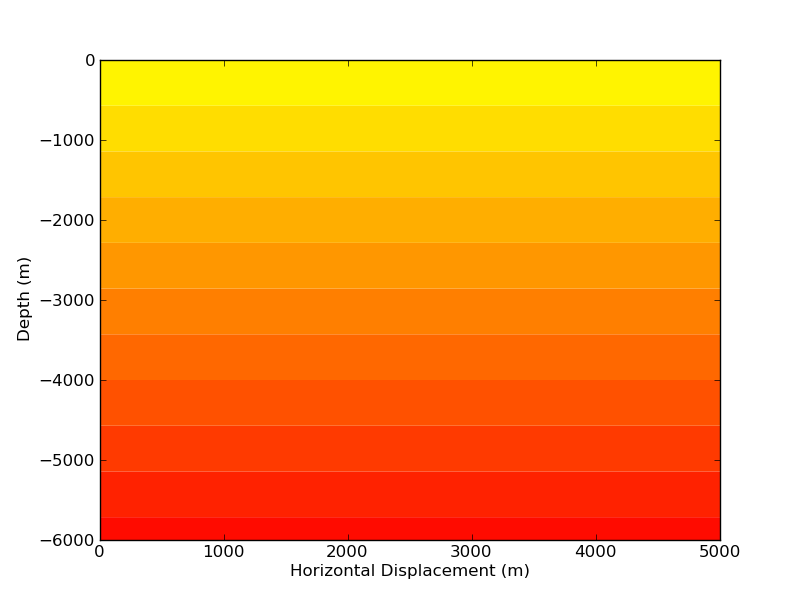
\includegraphics[width=4.in]{figures/simpleheat}}
\caption{Example 4b: Result of simple steady state heat problem.}
\label{fig:steady state heat}
\end{figure}


\section{The Steady-state Heat Equation}
\sslist{example04b.py, cblib}
A temperature equilibrium or steady state is reached when the temperature
distribution in the model does not change with time. To calculate the 
the steady state solution the time derivative term in \refEq{eqn:Tform nabla}
needs to be set to zero;
\begin{equation}\label{eqn:Tform nabla steady}
-\nabla \cdot \kappa \nabla T = q\hackscore H
\end{equation}
This PDE is easier to solve than the PDE in \refEq{eqn:hdgenf2}, as no time
steps (iterations) are required. The \verb|D| term from \refEq{eqn:hdgenf2} is
simply dropped in this case.
\begin{python}
mypde=LinearPDE(domain)
mypde.setValue(A=kappa*kronecker(model), Y=qH)
\end{python}
The temperature at the top face of the domain is known as \verb|Ttop| (=$20 C$).
In \refSec{Sec:1DHDv0} we have 
already discussed how this constraint is added to the PDE:
\begin{python}
x=Solution(domain).getX()
mypde.setValue(q=whereZero(x[1]-sup(x[1])),r=Ttop)
\end{python}
Notice that we use the \verb|sup| function to calculate the maximum of $y$
coordinates of the relevant sample points.

In all cases so far we have assumed that the domain is insulated which
translates 
into a zero normal flux $-n \cdot \kappa \nabla T$, see \refEq{eq:hom flux}. In
the modeling
set-up of this chapter we want to set the normal heat flux at the bottom to
\verb|qin| while we still
maintain insulation at the left and right face. Mathematically we can express
this as the format
\begin{equation}
-n \cdot \kappa \nabla T = q\hackscore{S}
\label{eq:inhom flux}
\end{equation}
where $q\hackscore{S}$ is a function of its location on the boundary. Its value
becomes zero
for locations on the left or right face of the domain while it has the value
\verb|qin| at the bottom face.
Notice that the value of $q\hackscore{S}$ at the top face is not relevant as we
prescribe the temperature here.
We could define $q\hackscore{S}$ by using the masking techniques demonstrated
earlier. The tagging mechanism provides an alternative and in many cases more
convenient way of defining piecewise 
constant functions such as $q\hackscore{S}$. Recall now that the bottom face was
denoted with the name \verb|linebottom| when we defined the domain. 
We can use this now to create $q\hackscore{S}$;
\begin{python}
qS=Scalar(0,FunctionOnBoundary(domain))
qS.setTaggedValue("linebottom",qin)
\end{python}
In the first line \verb|qS| is defined as a scalar value over the sample points
on the boundary of the domain. It is
initialized to zero for all sample points. In the second statement the values
for those sample points which
on the line marked by \verb|linebottom| are set to \verb|qin|. 

The Neuman boundary condition assumed by \esc has the form
\begin{equation}\label{NEUMAN 2b}
n\cdot A \cdot\nabla u = y 
\end{equation}
In comparison to the version in \refEq{NEUMAN 2} we have used so far the right
hand side is now 
the new PDE coefficient $y$. As we have not specified $y$ in our previous
examples, \esc has assumed
the value zero for $y$. A comparison of \refEq{NEUMAN 2b} and \refEq{eq:inhom
flux} reveals that one need to
choose $y=-q\hackscore{S}$;
\begin{python}
qS=Scalar(0,FunctionOnBoundary(domain))
qS.setTaggedValue("linebottom",qin)
mypde.setValue(y=-qS)
\end{python}
To plot the results we are using the \modmpl library as shown \refSec{Sec:2DHD
plot}. For convenience
the interpolation of the temperature to a rectangular grid for contour plotting
is made available
via the \verb|toRegGrid| function in the \verb|cblib| module. Your result should
look similar to 
\reffig{fig:steady state heat}.

\begin{figure}[ht]
\centerline{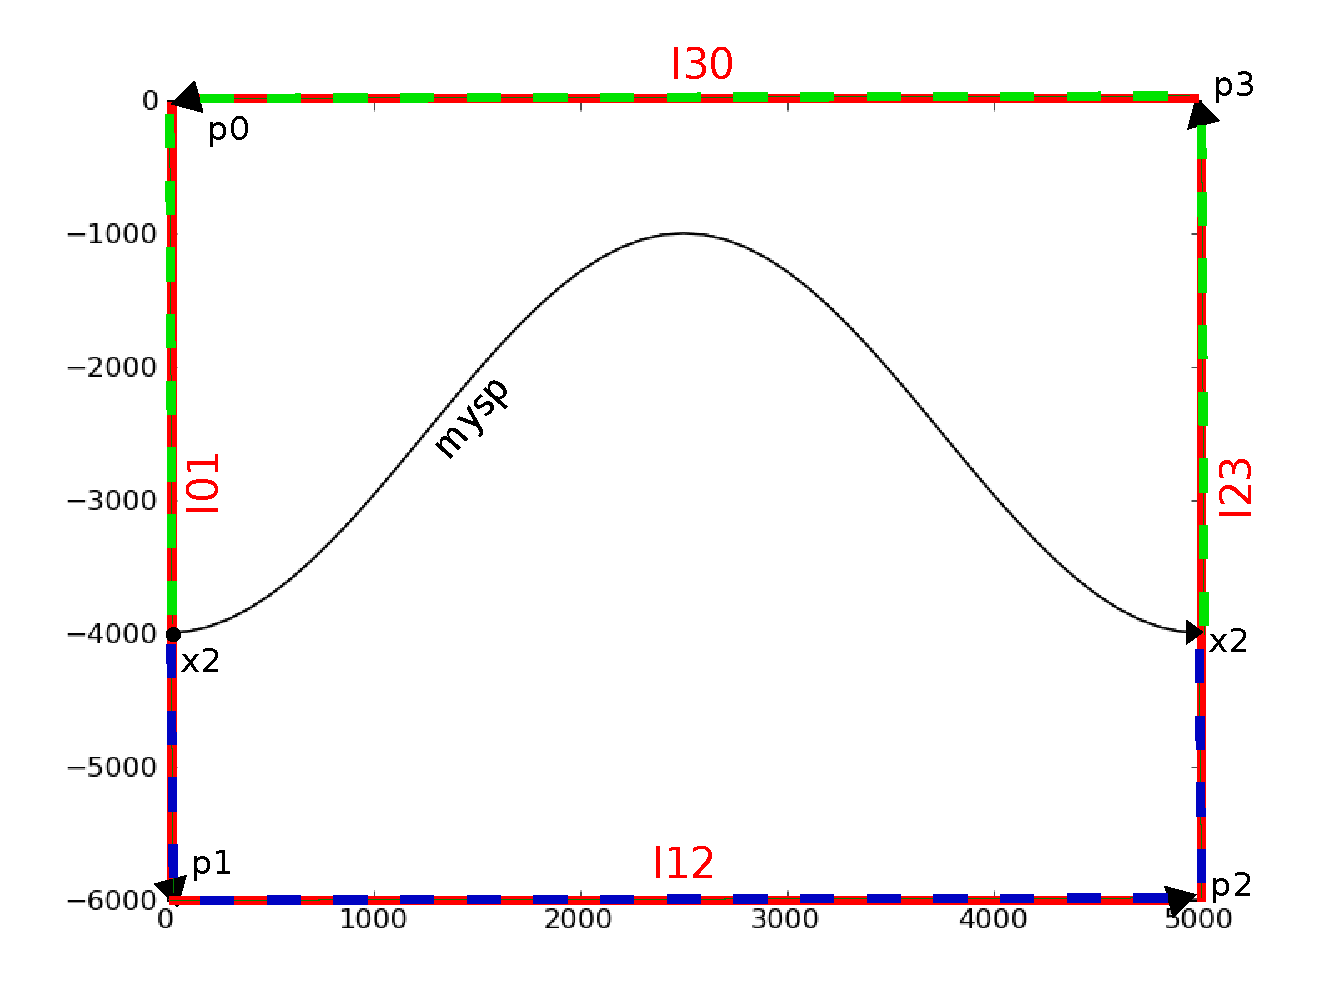
\includegraphics[width=4.in]{figures/anticlineheatrefraction}}
\caption{Example 5a: Heat refraction model with point and line labels.}
\label{fig:anticlinehrmodel}
\end{figure}

\begin{figure}[ht]
\centerline{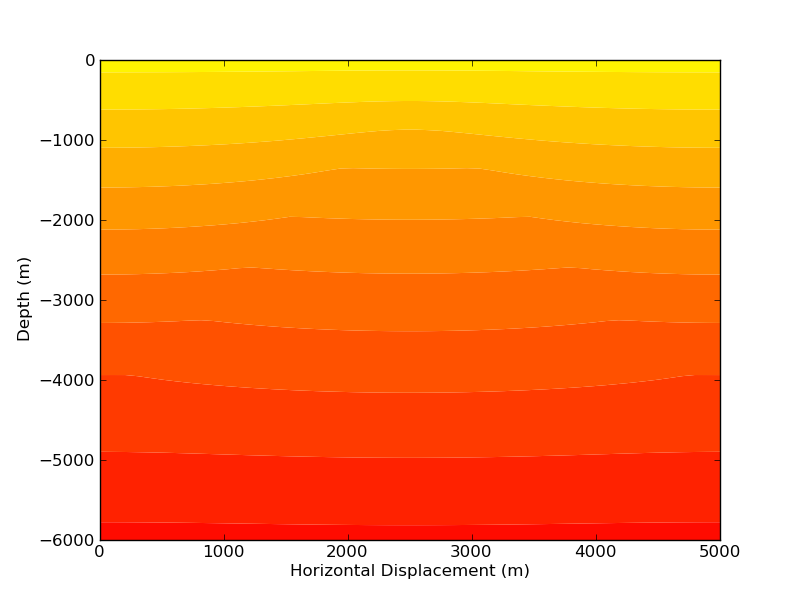
\includegraphics[width=4.in]{figures/heatrefraction}}
\caption{Example 5a: Temperature Distribution in the Heat Refraction Model.}
\label{fig:anticlinetemp}
\end{figure}

\section{Example 5: A Heat Refraction model}
\label{example5}
\sslist{example05a.py and cblib.py}
Our heat refraction model will be a large anticlinal structure that is subject
to a constant temperature at the surface and experiencing a steady heat flux at
it's base. Our aim is to show that the temperature flux across the surface is
not linear from bottom to top, but is in fact warped by the structure of the
model. The heat flow pattern demonstrates the dependence upon the material
properties and the shape of the interface.

The script of \refSec{example4} is modifed by subdividing the block into two
parts. The curve
separating the two blocks is given as a spline, see
\reffig{fig:anticlinehrmodel}. The data points
used to define the curve may be imported from a database of measurements
(\textit{e.g.} borehole depth data), but for simplicity it is assumed here that
the coordinates are
known in an analytic form.

There are two modes available in this example. When \verb modal=1 , this
indicates to the script that the model should be an anticline. Otherwise, when
\verb modal=-1 , thel model is a syncline. The modal operator simply changes the
orientation of the boundary function so that it is either upwards or downwards
curving. A \verb save_path  has also been defined so that we can easily separate
our data from other examples and our scripts. 

It is now possible to start defining our domain and boundaries. 

The curve defining our clinal structure is located approximately in the middle
of the domain and has a sinusoidal shape. We define the curve by generating
points at discrete intervals; $51$ in this case, and then create a smooth curve
through the points using the \verb Spline()  function.
\begin{python}
# Material Boundary
x=[ Point(i*dsp\
    ,-dep_sp+modal*orit*h_sp*cos(pi*i*dsp/dep_sp+pi))\
     for i in range(0,sspl)\
    ]
mysp = Spline(*tuple(x)) #*tuple() forces x to become a tuple
\end{python}
The start and end points of the spline can be returned to help define the
material boundaries.
\begin{python}
x1=mysp.getStartPoint()
x2=mysp.getEndPoint()
\end{python}
The top block or material above the clinal/spline boundary is defined in an
\textbf{anti-clockwise} manner by creating lines and then a closed loop. By
meshing the sub-domain we also need to assign it a planar surface. 
\begin{python}
# TOP BLOCK
tbl1=Line(p0,x1)
tbl2=mysp
tbl3=Line(x2,p3)
l30=Line(p3, p0)
tblockloop = CurveLoop(tbl1,tbl2,tbl3,l30)
tblock = PlaneSurface(tblockloop)
\end{python}
This process is repeated for every other sub-domain. In this example there is
only one other, the bottom block. The process is similar to the top block but
with a few differences. The spline points must be reversed by setting the spline
as negative.
\begin{python}
bbl4=-mysp
\end{python}
This reverse spline option unfortunately does not work for the getLoopCoords
command, however, the \modmpl polygon tool will accept clock-wise oriented
points so we can define a new curve.
\begin{python}
#clockwise check
bblockloop=CurveLoop(mysp,Line(x2,p2),Line(p2,p1),Line(p1,x1))
\end{python}
The last few steps in creating the domain require that the previously defined
domain and sub-domain points are submitted to generate a mesh that can be
imported into \esc.
To initialise the mesh it first needs some design parameters. In this case we
have 2 dimensions \verb dim  and a specified number of finite elements that need
to be applied to the domain \verb element_size  . It then becomes a simple task
of adding the sub-domains and flux boundaries to the design. Each element of our
model can be given an identifier which makes it easier to define the sub-domain
properties in the solution script. This is done using the 
\verb PropertySet()  function. The geometry and mesh are then saved so the \esc domain can be
created.
\begin{python}
# Create a Design which can make the mesh
d=Design(dim=2, element_size=200)
# Add the sub-domains and flux boundaries.
d.addItems(PropertySet("top",tblock),PropertySet("bottom",bblock),\
                   PropertySet("linebottom",l12))
# Create the geometry, mesh and \esc domain
d.setScriptFileName(os.path.join(save_path,"example05.geo"))
d.setMeshFileName(os.path.join(save_path,"example05.msh"))
domain=MakeDomain(d,optimizeLabeling=True)
\end{python}
The creation of our domain and its mesh is complete.

With the mesh imported it is now possible to use our tagging property to set up
our PDE coefficients. In this case $\kappa$ is set via the \verb
setTaggedValue()  function which takes two arguments, the name of the tagged
points and the value to assign to them. 
\begin{python}
# set up kappa (thermal conductivity across domain) using tags
kappa=Scalar(0,Function(domain))
kappa.setTaggedValue("top",2.0*W/m/K)
kappa.setTaggedValue("bottom",4.0*W/m/K)
\end{python}
No further changes are required to the PDE solution step, see
\reffig{fig:anticlinetemp} for the result. 

\begin{figure}
\centering
    \subfigure[Temperature Depth
Profile]{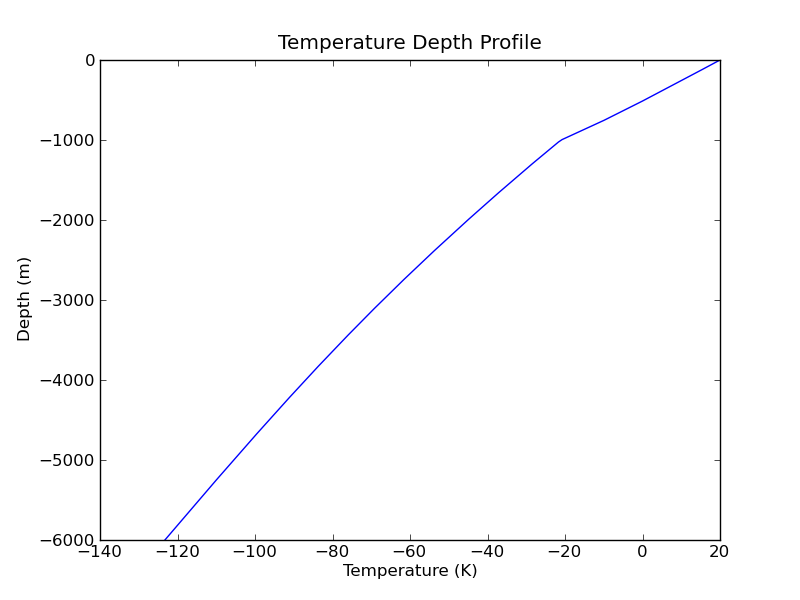
\includegraphics[width=3in]{figures/heatrefractiontdp.png}\label{
fig:tdp}}
    \subfigure[Temperature Gradient Depth
Profile]{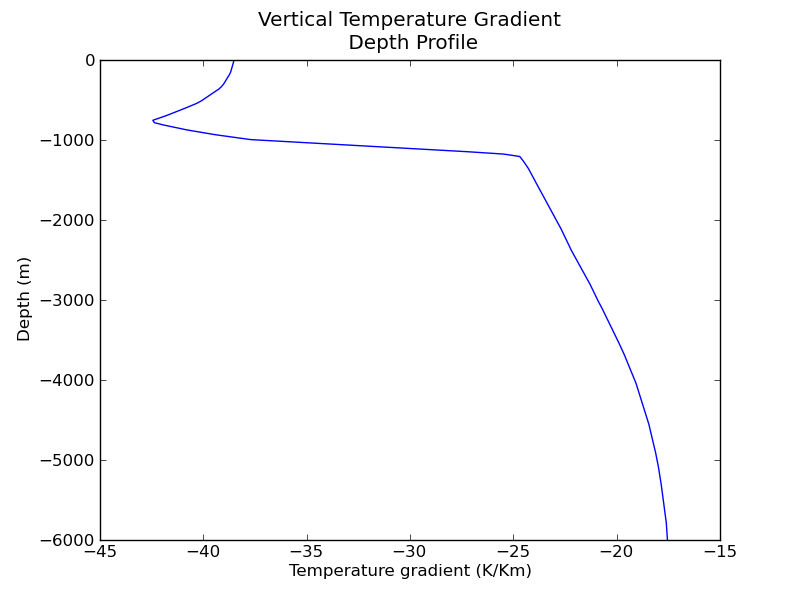
\includegraphics[width=3in]{figures/heatrefractiontgdp.png}\label{
fig:tgdp}}
    \subfigure[Thermal Conductivity
Profile]{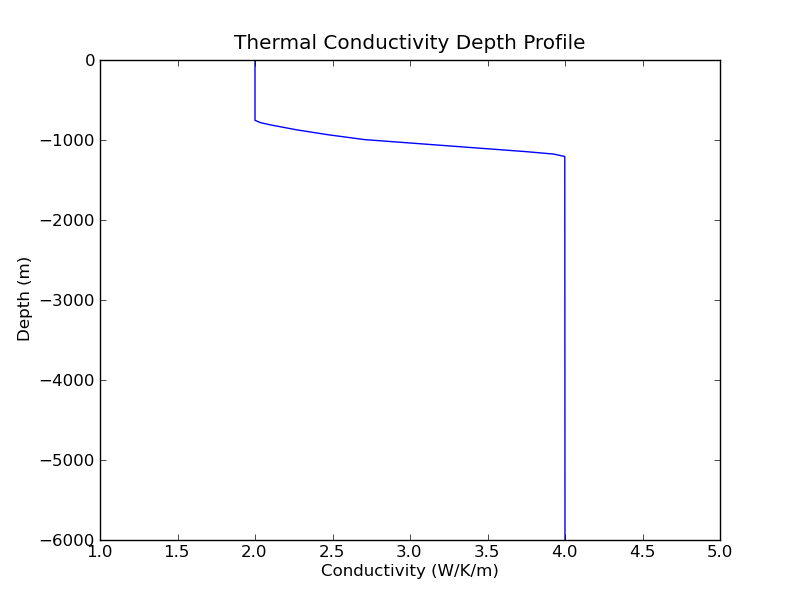
\includegraphics[width=3in]{figures/heatrefractiontcdp.png}\label{
fig:tcdp}}
    \subfigure[Heat Flow Depth
Profile]{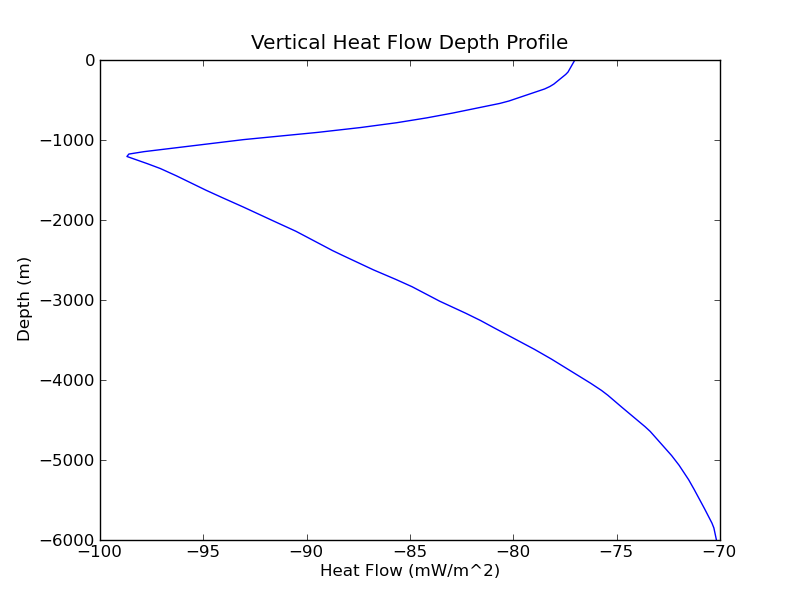
\includegraphics[width=3in]{figures/heatrefractionhf.png}\label{fig:hf}
}
  \caption{Example 5b: Depth profiles down centre of model.}
  \label{figs:dps}
\end{figure}

\section{Line profiles of 2D data}
\sslist{example05b.py and cblib.py}
We want to investigate the profile of the data of the last example. 
We are particularly interested in the depth profile of the heat flux which is
the second component of $-\kappa \nabla T$. The script from the previous section
is extended
to show how a vertical profile can be plotted.

The first important piece of information, is that \esc assumes that $-\kappa
\nabla T$ is not smooth and
that the point values of this solution are defined at numerical interpolation points. This assumption
is reasonable as
the flux is the product of the piecewise constant function $\kappa$ and 
the gradient of the temperature $T$ which has a discontinuity at the rock
interface. 
Before plotting this function we need to smooth the solution using the 
\verb|Projector()| class;
\begin{python}
from esys.escript.pdetools import Projector
proj=Projector(domain)
qu=proj(-kappa*grad(T))
\end{python}
The \verb|proj| object provides a mechanism to distribute values given at the
numerical interpolation points to the nodes
of the FEM mesh - the heat flux in this example. \verb|qu| has the same function
space
as the temperature \verb|T|. The smoothed flux is interpolated 
to a regular $200\times 200$ grid via;
\begin{python}
xiq,yiq,ziq = toRegGrid(qu[1],200,200)
\end{python}
using the \verb|toRegGrid| function from the cookbook library which we are using
for the contour plot.
At return \verb|ziq[j,i]| is the value of vertical heat flux at point 
(\verb|xiq[i]|,\verb|yiq[j]|). We can easily create deep profiles now by
plotting slices \verb|ziq[:,i]| over \verb|yiq|. The following script
creates a deep profile at $x_{0}=\frac{width}{2}$;
\begin{python}
cut=int(len(xiq)/2)
pl.plot(ziq[:,cut]*1000.,yiq)
pl.title("Vertical Heat Flow Depth Profile")
pl.xlabel("Heat Flow (mW/m^2)")
pl.ylabel("Depth (m)")
pl.savefig(os.path.join(save_path,"hf.png"))
\end{python}
This process can be repeated for various variations of the solution. In this
case we have temperature, temperature gradient, thermal conductivity and heat
flow \reffig{figs:dps}.

\begin{figure}[ht]
\centerline{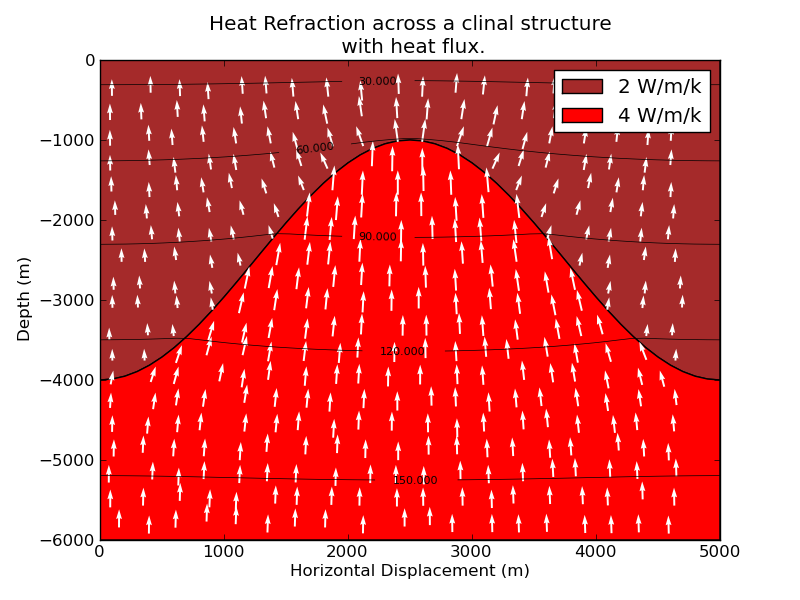
\includegraphics[width=5.in]{figures/heatrefractionflux}}
\caption{Example 5c: Heat refraction model with gradient indicated by vectors.}
\label{fig:hr001qumodel}
\end{figure}

\section{Arrow plots in \mpl}
\sslist{example05c.py and cblib.py}
The distribution of the flux $-\kappa \nabla T$ is now visualised over the
domain 
and the results are plotted in \reffig{fig:hr001qumodel}. 
The plot puts together three components. A contour plot of the temperature,
a colored representation of the two sub-domains where colour represents the
thermal conductivity 
in the particular region and finally the arrows representing the local direction
of the steepest gradient of the flux.

Contours have already been discussed in \refSec{Sec:2DHD plot}. To show
sub-domains, 
we need to go back to \pycad data to get the points used to describe the
boundary of the 
sub-domains. We have created the \verb|CurveLoop| class object 
\verb|tblockloop| to define the boundary of the upper sub-domain. 
We use the \verb|getPolygon()| method of \verb|CurveLoop| to get
access to the \verb|Point|s used top define the boundary. The statement
\begin{python}
[ p.getCoordinates() for p in tblockloop.getPolygon() ])
\end{python}
creates a list of the node coordinates of all the points in question. In order 
to simplify the selection of the $x$ and $y$ coordinates the list is converted 
into \modnumpy array. To add the area colored in brown to the plot we use; 
\begin{python}
import pylab as pl
import numarray as np
tpg=np.array([p.getCoordinates() for p in tblockloop.getPolygon() ])
pl.fill(tpg[:,0],tpg[:,1],'brown',label='2 W/m/k',zorder=-1000)
\end{python}
The same code is applied to \verb|bblockloop| to create the red area for this
sub-domain.

To plot vectors representing the flux orientation we use the 
\verb|quiver| function in \pylab. The function places vectors at locations in
the domain.
For instance one can plot vectors at the locations of the sample points used by
\esc 
to represent the flux \verb|-kappa*grad(T)|. As a vector is plotted at each
sample point one typically ends
up with two many vectors. So one needs to select a subset of points:
First we create a coarse grid of points on a rectangular mesh, e.g. $20 \times
20$ points. Here we choose a grid of points which are located at the center of a
\verb|nx| $\times$ \verb|ny| grid;
\begin{python}
dx = width/nx # x spacing
dy = depth/ny # y spacing
grid = [ ] # the grid points
for j in xrange(0,ny-1):
    for i in xrange(0,nx-1):
           grid.append([dx/2+dx*i,dy/2+dy*j])
\end{python}
With the \verb|Locator|  function \esc provides a mechanism to identify sample
points that are closest 
to the the grid points we have selected and to rettieve the data at these data
points; 
\begin{python}
from esys.escript.pdetools import Locator
flux=-kappa*grad(T)
fluxLoc = Locator(flux.getFunctionSpace(),grid)
subflux= fluxLoc(flux) 
\end{python}
\verb|subflux| gives now a list of flux component at certain sample points. To
get the 
list of the sample point coordinates one can use the \verb|getX()| method of
the 
\verb|Locator|;
\begin{python}
subfluxloc = fluxLoc.getX()
\end{python}
To simplify the selection of $x$ and $y$ components it is convenient 
to transform \verb|subflux| and \verb|subfluxloc| to \numpy arrays
\verb|xflux|, \verb|flux|.
This function is implemented in the \verb|subsample| 
in the  \file{clib.py} file so we can use it in other examples. One can easily
use this function 
to create a vector plot of the flux;
\begin{python}
from cblib import subsample
xflux, flux=subsample(-kappa*grad(T), nx=20, ny=20)
pl.quiver(xflux[:,0],xflux[:,1],flux[:,0],flux[:,1], angles='xy',color="white")
\end{python}
We add title and labels;
\begin{python}
pl.title("Heat Refraction across a clinal structure.")
pl.xlabel("Horizontal Displacement (m)")
pl.ylabel("Depth (m)")
pl.title("Heat Refraction across a clinal structure \n with gradient quivers.")
pl.savefig(os.path.join(saved_path,"flux.png"))
\end{python} 
to get the desired result, see \reffig{fig:hr001qumodel}.

\begin{figure}[ht]
\centerline{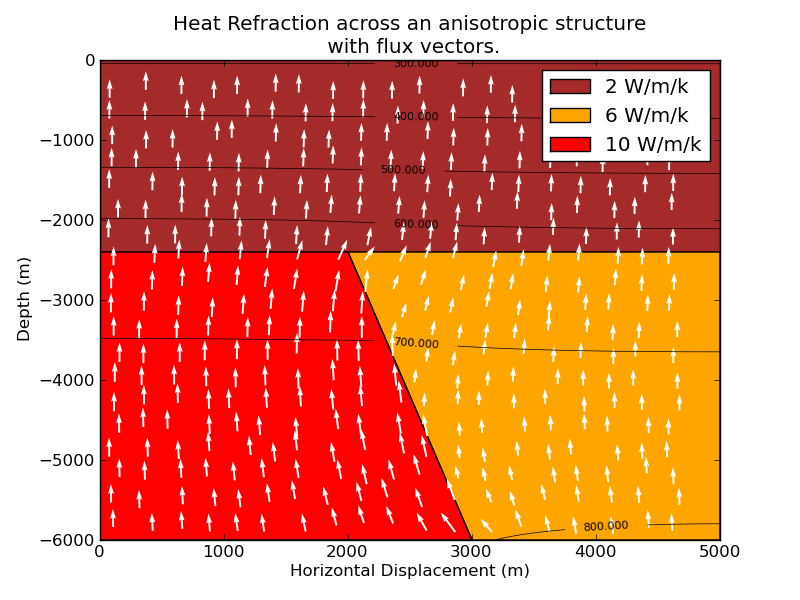
\includegraphics[width=4.in]{figures/heatrefraction2flux}}
\caption{Example 6: Heat refraction model with three blocks and heat flux.}
\label{fig:hr002qumodel}
\end{figure}

\section{Example 6:Fault and Overburden Model}
\sslist{example06.py and cblib.py}
A slightly more complicated model can be found in the examples
\textit{heatrefraction2_solver.py} where three blocks are used within the model,
see~\reffig{fig:hr002qumodel}. It is left to the reader to work through this
example.


